\documentclass[a4paper,11pt]{article}

\usepackage[english]{babel}
\usepackage{float}
\usepackage{graphicx}
\usepackage{amsmath,amsthm}
\usepackage{gensymb}
\usepackage{amssymb}
\usepackage[margin=2.cm]{geometry}
\usepackage{pstricks-add}	%for geometric diagrams
\usepackage{chemfig}	%for structural formulae
\usepackage{tabularx}	%for better tables
\usepackage{booktabs}	%for better tables
\usepackage[makeroom]{cancel}	%for cancelling lines
\usepackage{hyperref}	%hyperlinks
\usepackage{mathrsfs}
\usepackage{mathtools}
\usepackage{epigraph}	%quotes
\usepackage{lastpage}
\usepackage{multicol}	%column environments
\usepackage{fancyhdr}	%headers
\usepackage[at]{easylist}	%easy lists
\usepackage{wasysym}
\usepackage{wrapfig}	%wrap figures in text
\usepackage{subfig}		%subfigures
\usepackage{tikz}

\allowdisplaybreaks
\newcommand\numberthis{\addtocounter{equation}{1}\tag{\theequation}}
\setlength{\epigraphwidth}{7.7cm}
\setlength{\tabcolsep}{10pt}

% bracket group shorthands
\newcommand{\abs}[1]{\left|#1\right|}
\newcommand{\set}[1]{\left\{#1\right\}}

% common sets
\newcommand{\R}{\mathbb{R}}
\newcommand{\Cmplx}{\mathbb{C}}
\newcommand{\Q}{\mathbb{Q}}
\newcommand{\Z}{\mathbb{Z}}
\newcommand{\N}{\mathbb{N}}

% derivative shorthands
\newcommand{\diff}[2]{\frac{\mathrm{d}#1}{\mathrm{d}#2}}
\newcommand{\pdiff}[2]{\frac{\partial #1}{\partial #2}}
\newcommand{\ndiff}[3]{\frac{\mathrm{d}^{#3}#1}{\mathrm{d}#2^{#3}}}
\newcommand{\npdiff}[3]{\frac{\partial^{#3} #1}{\partial #2^{#3}}}

% theorem environments
\newtheorem*{definition*}{Definition}
\newtheorem*{lemma*}{Lemma}
\newtheorem{theorem}{Theorem}
\newtheorem*{theorem*}{Theorem}
\newtheorem*{corollary*}{Corollary}
\newtheorem{example}{Example}
\newtheorem*{remark}{Remark}

\DeclareMathOperator{\bdy}{Bdy}
\DeclareMathOperator{\interior}{Int}

% header
\pagestyle{fancy}
\lhead{Problem Set 1}
\rhead{Year 11 2018}

%\title{Problem Set 1}
%\date{\today}
%\author{Daniel Czapski}

\begin{document}
	\section*{Essential Revision Problems -- Set 1 -- Calculus, Trigonometry, Plane Geometry}
	\subsection*{Question 1: 1992 Q4 c.}
	
	\begin{center}
	\begin{tikzpicture}
	\draw (0,0) ellipse (1 and 2);
	\draw (6,-2) to [out=0,in=0] (6,2);
	\draw[dashed] (6,-2) to [out=180,in=180] (6,2);
	\draw (0,-2) -- (6,-2);
	\draw (0,2) -- (6,2);
	\draw[dashed] (0,-2) -- (3,2);
	
	\draw[->] (0,0) -- (0,2);
	\draw (0,-2.7) -- (0,-2.3);
	\draw (6,-2.7) -- (6,-2.3);
	\draw (0,-2.5) -- (2.75,-2.5);
	\draw (3.25,-2.5) -- (6,-2.5);
	\draw (0,2.7) -- (0,2.3);
	\draw (3,2.7) -- (3,2.3);
	\draw (0,2.5) -- (1.25,2.5);
	\draw (1.75,2.5) -- (3,2.5);
	
	\draw[fill=black] (0,0) circle [radius=0.075cm];
	\draw[fill=black] (0,-2) circle [radius=0.075cm];
	\draw[fill=black] (3,2) circle [radius=0.075cm];
	
	\node [above] at (-0.15,-1.9) {$A$};
	\node [above right] at (3,2) {$B$};
	\node [right] at (1.5,0) {$d$};
	\node [left] at (0,1) {$r$};
	\node at (3,-2.5) {$l$};
	\node at (1.5,2.5) {$\dfrac{l}{2}$};
	\end{tikzpicture}
	\end{center}
	
	Consider a cylindrical barrel of length $l$ and radius $r$. The point $A$ is at one end of the barrel, at the very bottom of the rim. The point $B$ is at the very top of the barrel, half-way along its length. The length of $AB$ is $d$.\\
	
	\begin{easylist}
		\ListProperties(Start1=1,Numbers1=r,Margin=1cm,FinalMark1={)},Space*=0.15cm)
		@ Show that the volume of the barrel is
		$$
		V = \frac{\pi l}{4}\left(d^2-\frac{l^2}{4}\right).
		$$
		@ Find $l$ in terms of $d$ if the barrel has a maximum volume for the given $d$.
	\end{easylist}

	\subsection*{Question 2: 1993 Q2 a.}
	Prove
	$$
	\frac{\sin A}{\cos A + \sin A} + \frac{\sin A}{\cos A - \sin A} = \tan 2A.
	$$
	
	\subsection*{Question 3: 1993 Q4 a.}
	\begin{center}
		\begin{tikzpicture}[scale=0.85]
		\draw (0,0) circle [radius=3cm];
		\draw (0,3) -- (0,-3);
		\draw[domain=0:7.819] plot (\x,-0.7673*\x+3);
		\draw (0,-3) -- (9,-3);
		\draw[dashed] (0,-3) -- (2.893,0.7765);
		\draw[domain=2.2945:3.9097] plot (\x,-3.7145*\x+11.522);
		\draw (1.233,-3) arc (0:52.5:1.233);
		
		\draw[fill=black] (0,0) circle [radius=0.075cm];
		
		\node[above] at (0,3) {$A$};
		\node[left] at (0,0) {$O$};
		\node[below] at (0,-3) {$B$};
		\node[below] at (3.9097,-3) {$F$};
		\node[below] at (7.819,-3) {$D$};
		\node[below] at (9,-3) {$C$};
		\node[above right] at (2.893,0.7765) {$E$};
		\node[above] at (2.2945,3) {$G$};
		\node at (0.8,-2.6) {$\alpha$};
		\end{tikzpicture}
	\end{center}
	In the diagram, $AB$ is a diameter of the circle, centre $O$, and $BC$ is tangential to the circle at $B$. The line $AED$ intersects the circle at $E$ and $BC$ at $D$. The tangent to the circle at $E$ intersects $BC$ at $F$. Let $\angle EBF=\alpha$.
    \pagebreak
	
	\begin{easylist}
	\ListProperties(Start1=1,Numbers1=r,Margin=1cm,FinalMark1={)},Space*=0.5cm)
	@ Copy the diagram into your workbook.
	@ Prove that $\angle FED=90-\alpha$.
	@ Prove that $BF=FD$.
	\end{easylist}

	\subsection*{Question 4: 1994 Q5 c, i--ii.}
	\begin{center}
		\begin{tikzpicture}[scale=1.2,yscale=4]
		\draw[->] (0,-0.25) -- (0,1.1) node[left] {$y$};
		\draw[->] (-5,0) -- (5,0) node[below] {$x$};
		\draw[domain=-5:5] plot (\x,0.03125*\x*\x);
		\draw (0,0.78125) ellipse (5 and 0.1);
		\draw[dashed] (-0.15,0.78125) node[left] {$h$} -- (5,0.78125);
		\draw[->] (-3.5,1) node[above left] {$S$} -- (-2.75,0.78125);
		
		\node[below left] at (0,0) {$O$};
		\node at (4,0.25) {$x^2=32y$};
		%\node at (-3.5,1) {$S$};
		\end{tikzpicture}
	\end{center}
The diagram represents the water in the dam on a farm. The curve is described by the equation $x^2=32y$. The depth of the water is $h$ meters, the volume of water in the dam in cubic metres is given by $V = 16\pi h^2$ and the surface area of the water is $S$ square metres. The water in the dam evaporates according to the rule 
$$
\diff{V}{t} = -kS
$$
where $k$ is a positive constant and $t$ is the time in hours. 

\begin{easylist}
	\ListProperties(Start1=1,Numbers1=r,Margin=1cm,FinalMark1={)},Space*=0.5cm)
	@ Describe in words what the rule says about the rate of evaporation.
	@ Show that $\diff{h}{t} = -k$.
\end{easylist}

\subsection*{Question 5*: 1994 Q7 c.}
Uluru is a large rock on flat ground in Central Australia. Three tourists, $A$, $B$ and $C$ are observing Uluru from the ground. $A$ is due North of Uluru, $C$ is due East of Uluru and $B$ is on the line-of-sight from $A$ to $C$ and between them\footnote{i.e. on the line from $A$ to $C$.}. The angles of elevation to the summit of Uluru from $A$, $B$ and $C$ are 26\degrees, 28\degree and 30\degree respectively.\\

\noindent Determine the bearing of $B$ from Uluru.
\pagebreak

\subsection*{Question 6: 1995 Q4 a--e.}
Consider the real-valued function $f$ such that
$$
f(x) = \frac{e^x}{3+e^x}.
$$
Note that $e^x$ is always positive, $f(x)$ is defined for all real $x$, and the following important facts:
\begin{align*}
\diff{}{x}\left(e^x\right) = e^x && e^x = y \iff x = \log_e(y) = \ln(y).
\end{align*}
\begin{easylist}
	\ListProperties(Start1=1,Numbers1=l,Margin=1cm,FinalMark1={)},Space*=0.5cm)
	@ Show that $f(x)$ has no stationary points. Hint: use the first important fact. (2)
	@ Find the coordinates of the point of inflexion, given that
	$$
	f''(x) = \frac{3e^x(3-e^x)}{(3+e^x)^3}.
	$$
	Hint: use the second important fact. (1)
	@ Show that $0<f(x)<1$ for all $x$. (2)
	@ Describe the behaviour of $f(x)$ for very large positive and very large negative values of $x$, i.e. as $x\to\infty$ and $x\to-\infty$. (2)
	@ Sketch the curve $y=f(x)$. (2)
\end{easylist}

\subsection*{Question 7: 2000 Q3 a.}
Use the definition
$$
f'(a) = \lim\limits_{h\to 0}\frac{f(a+h)-f(a)}{h}
$$
to find the derivative of $x^3$ where $x=a$. (2)

\subsection*{Question 8*: 2003 Q6 b.}
\begin{center}
	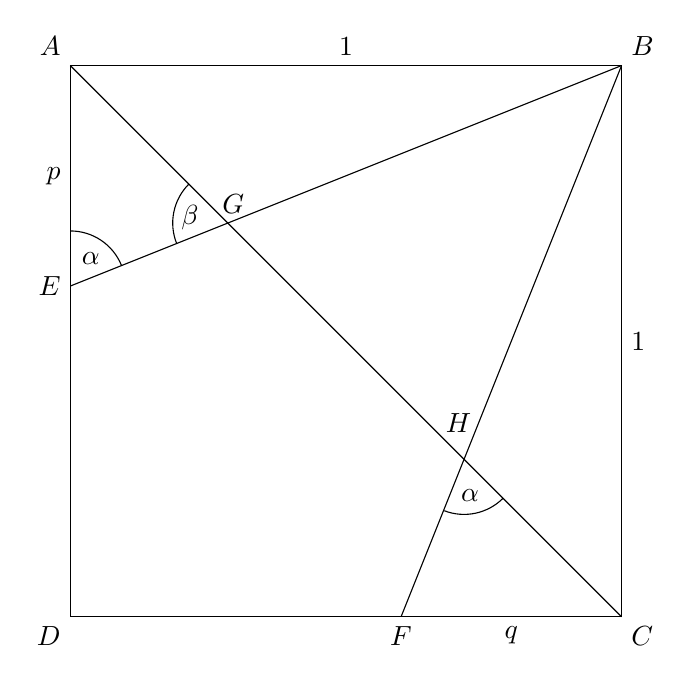
\begin{tikzpicture}[scale=7]
	\draw (0,0) rectangle (1,1);
	\draw (0,1) -- (1,0);
	\draw (0,0.6) -- (1,1);
	\draw (0.6,0) -- (1,1);
	
	\draw (0,0.7) arc (90:22:0.1);
	\draw (0.214989,0.785011) arc (135:202:0.1);
	\draw (0.785011,0.214989) arc (-45:-111:0.1);
	
	\node[above left] at (0,1) {$A$};
	\node[left] at (0,0.8) {$p$};
	\node[left] at (0,0.6) {$E$};
	\node[below left] at (0,0) {$D$};
	\node[below] at (0.6,0) {$F$};
	\node[below] at (0.8,0) {$q$};
	\node[below right] at (1,0) {$C$};
	\node[right] at (1,0.5) {$1$};
	\node[above right] at (1,1) {$B$};
	\node[above] at (0.5,1) {$1$};
	\node[above] at (0.2957,0.7143) {$G$};
	\node[above] at (0.7043,0.3157) {$H$};
	
	\node at (0.037,0.65) {$\alpha$};
	\node at (0.217,0.724) {$\beta$};
	\node at (0.725,0.22) {$\alpha$};
	\end{tikzpicture}
\end{center}
In the diagram, $ABCD$ is a unit square. Points $E$ and $F$ are chosen on $AD$ and $DC$ respectively, such that $\angle AEG=\angle FHC$, where $G$ and $H$ are the points at which $BE$ and $BF$ respectively cut the diagonal $AC$.\\

\noindent Let $AE=p$, $FC=q$, $\angle AEG=\alpha$ and $\angle ABE=\beta$.

\begin{easylist}
	\ListProperties(Start1=1,Numbers1=r,Margin=1cm,FinalMark1={)},Space*=0.5cm)
	@ Express $\alpha$ in terms of $p$ and $\beta$ in terms of $q$. (2)
	@ Prove that $p+q=1-pq$. (2)
	@ Show that the area of the quadrilateral $EBFD$ is given by
	$$
	1-\frac{p}{2}+\frac{p-1}{2(p+1)}.\quad (1)
	$$
	@ What is the maximum value of the area of $EBFD$? (2)
\end{easylist}

\subsection*{Question 9: 2004 Q6 a.}
\begin{center}
	\begin{tikzpicture}
	%\draw (0,-4) grid (12,4);
	\draw (0,0) circle [radius=4cm];
	\draw (-1.3681,-3.75877) node[below left] {$D$} -- (9,-2) node[right] {$F$};
	\draw (0.3486,3.9848) node[above left] {$A$} -- (9,-2);
	\draw (-1.3681,-3.75877) -- (3.60574,1.73166) node[above right] {$B$};
	\draw (0.3486,3.9848) -- (2.53008,-3.09818) node[below right] {$C$};
	\draw (-1.3681,-3.75877) -- (0.3486,3.9848);
	
	\node[left] at (1.69287,-0.379876) {$E$};
	\end{tikzpicture}
\end{center}
The points $A,B,C$ and $D$ are placed on a circle of radius $r$ such that $AC$ and $BD$ meet at $E$. The lines $AB$ and $DC$ are produced to meet $F$ and $BECF$ is a cyclic quadrilateral.

\begin{easylist}
	\ListProperties(Start1=1,Numbers1=r,Margin=1cm,FinalMark1={)},Space*=0.5cm)
	@ Find the size of $\angle DBF$, giving reasons for your answer. (2)
	@ Find an expression for the length of $AD$ in terms of $r$. (1)
\end{easylist}

\subsection*{Question 10: 2008 Q5 c.}
\begin{center}
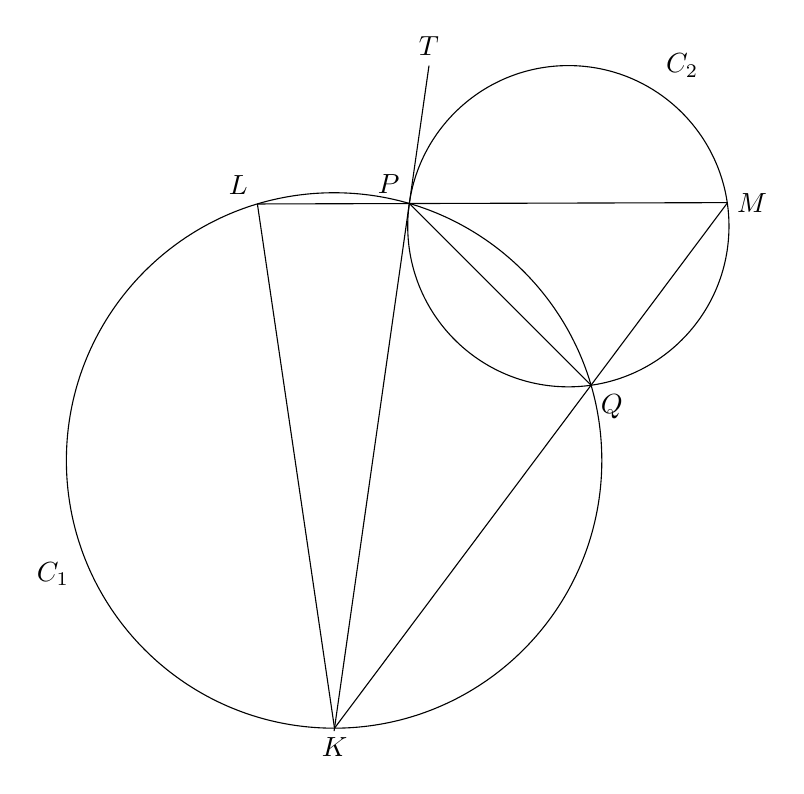
\begin{tikzpicture}[scale=1.7]
\draw (0,0) circle [radius=2cm];
\draw (1.75,1.75) circle [radius=1.2cm];
%(1.91941,0.56218)
\draw (1.91941,0.56218) node[below right] {$Q$} -- (0.56218,1.91941) node[above left] {$P$};
\draw[domain=0:0.708983] plot (\x,7.012467*\x-2.02172);
\draw[domain=0.0031:2.93699] plot (\x,1.33695*\x-2.004);
\draw[domain=-0.573:2.93699] plot (\x,0.002863*\x+1.9178);
\draw (-0.573,1.91616) -- (0.0031,-2);

\node[right] at (2.93699,1.92621) {$M$};
\node[above left] at (-0.573,1.91616) {$L$};
\node[below] at (0.0031,-2) {$K$};
\node[above] at (0.708983,2.95) {$T$};
\node at (-2.1,-0.85) {$C_1$};
\node at (2.6,2.95) {$C_2$};
\end{tikzpicture}
\end{center}
Two circles $C_1$ and $C_2$ intersect at $P$ and $Q$ as show in the diagram. The tangent $TP$ to $C_2$ meets $C_1$ at $K$. The line $KQ$ meets $C_2$ at $M$. The line $MP$ meets $C_1$ at $L$.\\

\noindent Prove that $\triangle PKL$ is isosceles. (3)

\subsection*{Question 11: 2009 Q3 c.}
\begin{easylist}
	\ListProperties(Start1=1,Numbers1=r,Margin=1cm,FinalMark1={)},Space*=0.5cm)
	@ Prove that
	$$
	\tan^2\theta = \frac{1-\cos 2\theta}{1+\cos 2\theta}
	$$
	provided that $\cos 2\theta\neq -1$. (2)
	@ Hence, find the exact value of $\tan 22.5\degree$. (1)
\end{easylist}

\subsection*{Question 12: 2009 Q4 b.}
Consider the function $f$ given by $f(x) = \dfrac{x^4+3x^2}{x^4+3}$.
\begin{easylist}
	\ListProperties(Start1=1,Numbers1=r,Margin=1cm,FinalMark1={)},Space*=0.5cm)
	@ Show that $f(x)$ is an even function. (1)
    @ What is the equation of the horizontal asymptote to the graph $y=f(x)$? (1)
    @ Find the $x-$coordinates of all stationary points for the graph $y=f(x)$. (3)
    @ Sketch the graph $y=f(x)$. You are not required to find any points of inflexion. (2)
\end{easylist}
\end{document}